\documentclass{report}

\input{preamble}
\input{macros}
\input{letterfonts}

\usepackage{tikz}
\usepackage{tikz-3dplot}
\usepackage{amsmath}
\usepackage{pgfplots}
\usepackage{smartdiagram}
\usepackage{graphicx}
\usepackage{chemfig}

\usepackage{amssymb}  % For additional symbols if needed
\usesmartdiagramlibrary{additions}

\title{\Huge{CASCH 131 }\\ \Large{John Caradonna}}
\author{\huge{Giacomo Cappelletto}}
\date{3/9/24}

\begin{document}


\maketitle
\newpage
\pdfbookmark[section]{\contentsname}{toc}
\tableofcontents
\pagebreak

\chapter{Atomic Theory and the Nature of Modern Chemistry}

\section{1.1 - The Nature of Modern Chemistry}

\dfn{Conservation of Energy and Mass}{
	Energy and mass are conserved in ordinary chemical reactions.
	The total mass of the products equals the total mass of the reactants.
}

\thm{Macroscopic and Nanoscopic Length Scales}{
	Chemical reactions occur on the scale of nanometers, yet are observed in laboratories on scales of grams and centimeters.
}


\section{The Atom in Modern Chemistry}

\nt{Modern Chemistry Timeline}{
	Modern chemistry is approximately 300 years old, with its roots dating back to the late 18th and early 19th centuries. Several foundational laws and principles emerged during this period, forming the basis of modern chemical science.
}

\subsection{Lavoisier: Conservation of Mass and Energy}

\dfn{Law of Conservation of Mass and Energy}{
	Antoine Lavoisier (1743–1794) formulated the Law of Conservation of Mass, which states that in a chemical reaction, mass is neither created nor destroyed. This principle was later extended to include energy, particularly after the development of modern physics.
}

\nt{Note on Lavoisier's Contribution}{
	Lavoisier's discovery revolutionized chemistry by providing a quantitative approach to chemical reactions. He is often called the "Father of Modern Chemistry."
}

\subsection{Proust: Law of Constant Composition}

\dfn{Law of Constant Composition (Definite Proportions)}{
	Joseph Proust (1754–1826) established the Law of Constant Composition, which states that a given chemical compound always contains its component elements in a fixed ratio by mass, regardless of its source or method of preparation.
}

\nt{Proust's Discovery}{
	This law was critical in distinguishing compounds from mixtures and emphasized the fixed, predictable nature of chemical compounds.
}

\subsection{Dalton: Law of Multiple Proportions}

\dfn{Law of Multiple Proportions}{
	John Dalton (1766–1844) introduced the Law of Multiple Proportions, which states that when two elements form more than one compound, the masses of one element that combine with a fixed mass of the other are in ratios of small whole numbers.
}

\nt{Example of Dalton's Law}{
	For example, carbon and oxygen form two compounds: carbon monoxide (CO) and carbon dioxide (CO$_2$). The mass ratio of oxygen in CO$_2$ to CO is 2:1.
}

\subsection{Gay-Lussac: Law of Combining Volumes}

\dfn{Law of Combining Volumes}{
	Joseph Louis Gay-Lussac (1778–1850) discovered that when gases react together at constant temperature and pressure, the volumes of the reactants and products (if gaseous) are in simple whole number ratios. This is known as the Law of Combining Volumes.
}

\nt{Gay-Lussac's Contribution}{
	This law played a crucial role in understanding the stoichiometry of gaseous reactions and helped pave the way for Avogadro's hypothesis.
}

\begin{center}
	\begin{tikzpicture}
		% Define the step size
		\def\step{1}

		% Draw the staircase
		\foreach \i in {0,...,4} {
				% Horizontal part of the step
				\draw[thick] (\i*\step, \i*\step) -- (\i*\step + \step, \i*\step);
				% Vertical part of the step
				\draw[thick] (\i*\step + \step, \i*\step) -- (\i*\step + \step, \i*\step + \step);
			}

	\end{tikzpicture}
\end{center}

\nt{Note on Visual Representation}{
	The staircase diagram illustrates the progressive development of chemistry over time, where each step represents a major discovery that builds on the previous one.
}

\section{1.2 - Elements: The Building Blocks of Matter}

\dfn{Mixtures and Compounds}{
	Mixtures can be separated by physical processes (e.g., filtration, distillation).
	Compounds are substances that can only be separated into simpler substances by chemical reactions.
}

\section{1.3 - Indirect Evidence for the Existence of Atoms}

\dfn{Dalton’s Atomic Theory}{
	Atoms are indivisible, retain their identity in chemical reactions, and combine in fixed whole-number ratios to form compounds.
}

\nt{Laws of Chemical Combination}{
	The laws of definite proportions and multiple proportions form the basis for determining chemical formulas.
}

\section{1.4 - The Physical Structure of Atoms}

\dfn{Cathode Ray Experiment}{
	Cathode rays are negatively charged particles (electrons) with a charge-to-mass ratio measured by Thomson and charge measured by Millikan.
}

\thm{Planetary Model of the Atom}{
	The scattering of alpha particles by gold established the planetary model: a dense nucleus surrounded by electrons.
}

\section{1.5 - Mass Spectrometry and Isotopes}

\nt{Relative Atomic Masses}{
	Elements have isotopes with different masses but identical chemical properties.
}

\section{1.6 - The Mole: Counting Molecules by Weighing}

\dfn{Avogadro’s Number}{
	$1 \, \text{mol} = 6.022 \times 10^{23}$ molecules.
	Molar mass is used to convert between mass, moles, and the number of molecules.
}

\chapter{19 - Nucleosynthesis of the Elements}

\section{19.1 - Mass-Energy in Nuclei}



\dfn{Nuclear Symbols}{

	\text{Number of nucleons A} \\
	\text{Number of protons Z}


	\[
		\prescript{\large A}{\large Z}{\mathrm{\large X}}
	\]
}


\section{19.2 - Nuclear Decay}

\dfn{Nuclear Decay Process}{


	\begin{center}
		\begin{tikzpicture}[node distance=2cm, auto]

			% Alpha Decay
			\node (start) at (0,0) {$\prescript{A}{Z}{\mathrm{X}}$};
			\node (alpha) [right=3cm of start] {$\prescript{A-4}{Z-2}{\mathrm{Y}} + \prescript{4}{2}{\mathrm{He}}$};
			\draw[->] (start) -- node[above] {Alpha Decay} (alpha);

			% Beta Decay
			\node (beta) [below=2cm of start] {$\prescript{A}{Z+1}{\mathrm{Y}} + \prescript{0}{-1}{\beta}$};
			\draw[->] (start) -- node[left] {Beta (Minus) Decay} (beta);

			% Gamma Decay
			\node (gamma) [below=2cm of alpha] {$\prescript{A}{Z}{\mathrm{X^*}} \rightarrow \prescript{A}{Z}{\mathrm{X}} + \gamma$};
			\draw[->] (start) -- node[right] {Gamma Decay} (gamma);

			% Add a box around the initial nucleus
			\draw[dashed] (start.north west) rectangle (start.south east);


		\end{tikzpicture}
	\end{center}
}

\dfn{Alpha Decay}{

	\textbf{Alpha decay} is the most common nuclear decay process. \\
	Alpha decay is most common in nuclei with atomic number greater than 82 (the highest binding energy per nuclei).

}

\dfn{Binding Energy per Nucleon}{

	\[
		\Delta E = \Delta m c^2
	\]

	\[
		\Delta E = M_{Z,A} - \left( M_{Z-2} + M_{2, \alpha} \right) c^2 > 0
	\]

	\[
		\text{If } \Delta E > 0 \quad \Rightarrow \quad \text{Decay Occurs}
	\]

	\[
		\text{If } \Delta E < 0 \quad \Rightarrow \quad \text{Stable}
	\]
	\centering
	\includegraphics[width=0.5\textwidth]{BEPN.png} % Adjust the width as needed
	\par\vspace{1em} % Adds a small space after the image

}

\dfn{Beta Decay}{

	\textbf{Beta decay} occurs when a nucleus emits or absorbs a neutron. \\
	Beta decay is very common in nuclei with atomic number less than 82.


}

\dfn{Gamma Decay}{
	\textbf{Gamma decay} occurs when a nucleus emits or absorbs a photon. \\
	Gamma decay is rare, but it can occur in high-energy nuclei.

	Photons of electromagnetic radiation that carry away excess energy when nuclei make $\gamma$ decay.

}
\section{19.6 - Nuclear Fusion}

\dfn{Origin of elements}{
	\textbf{Fusion of elements} involves 2 nuclei of very low A amalgamating to a form a more stable nucleus. \\
	Getting the A value nearer to 56 (the highest Binding Energy per nucleon).
}

\nt{Hubbles observaions of red shift in further galaxies and knowledge of fusion leads us to predict the existence of a singularity at the start of the current universe. What came before this is not known, but it is believed to be a singularity of the same type as the one at the end of the universe.\\
	\textbf{The Steady State model } states that the densigty of the expanding universe should remain constant. As the universe expands, the density of matter stays the same as more matter is created.
}

\dfn{Initial Events of Big Bang}{
	\begin{align*}
		{}^1_0 \text{n}                   & \rightarrow {}^1_1 \text{H} + e^- + \bar{\nu}_e \\
		{}^1_1 \text{H} + \nu_e           & \rightarrow {}^1_0 \text{n} + e^+               \\
		{}^1_1 \text{H} + {}^1_0 \text{n} & \rightarrow {}^2_1 \text{H} + \gamma            \\
		e^+ + e^-                         & \rightarrow \gamma + \gamma
	\end{align*}


	\begin{center}
		\textbf{Then}
	\end{center}

	\begin{align*}
		{}^1_1 \text{H} + {}^1_0 \text{n}  & \rightarrow {}^2_1 \text{H} + \gamma           \\
		{}^2_1 \text{H} + {}^2_1 \text{H}  & \rightarrow {}^3_2 \text{He} + {}^1_0 \text{n} \\
		{}^3_2 \text{He} + {}^1_0 \text{n} & \rightarrow {}^4_2 \text{He} + \gamma          \\
		{}^3_2 \text{He} + {}^1_1 \text{H} & \rightarrow {}^4_2 \text{He}
	\end{align*}
	\begin{center}
		\textbf{Helium 3 (werid particle due to its quantum behavior) and helium 4 are created $1/10$ of the time}
	\end{center}
}

\nt{The fusion of 1 gram  deuterium and helium 3 gives about 350 billion joules of energy. Reason for which we are trying to reproduce fission on earth}



\thm{Clusters}
{
	Ripples in the helium and tritium gas clouds form denser regions, which group further due to gravity $\rightarrow$ hydrogen burn $\rightarrow$ HE is formed in a star cycle of reactions (proton-proton cycle) and heavier elements move
	towards the center. Outer portions do proton-proton burn, inner denser portions of the start do helium burn.$\rightarrow$ Helium 4's combine to make Beryllium $^8_4\text{Be}$. Beryllium and Helium combine to make carbon 12 $^{12}_6\text{C}$. $\rightarrow$ CARBON CYCLE occurs as $^{12}_6\text{C}$ is the catalyst.
	By adding helium $^4_2\text{He}$ to all the elements in the dense cores, all the elements up to iron $^{56}_{26}\text{Fe}$ formed, and then stopped due to it having the highest binding energy per nucleon.
}

\thm{After Iron}{
	A 14 particle collision is needed to make elements after Iron, which is very unlikely.
	\[
		^{56}_{26}\text{Fe} + 13 ^1_0\text{n} \rightarrow ^{69}_{26}\text{Co} + e
	\]
}

\nt{Fusion only gets us 26 elements (in stars).}

\pagebreak

\chapter{Chemical Structures}

\section{Drawing Lewis Dot Structures}

Lewis dot structures are diagrams that show the bonding between atoms of a molecule and the lone pairs of electrons that may exist in the molecule. Here's a step-by-step guide on how to draw Lewis dot structures:

\subsection{Steps to Draw a Lewis Dot Structure}

1. \textbf{Count the Valence Electrons:}
Find the total number of valence electrons in the molecule by adding up the valence electrons of all atoms.

2. \textbf{Arrange the Atoms:}
Write the atoms in the molecule with the least electronegative atom as the central atom (except for hydrogen, which is always terminal).

3. \textbf{Form Bonds Between Atoms:}
Connect the atoms with single bonds. Each bond represents a pair of shared electrons.

4. \textbf{Distribute Remaining Electrons:}
Distribute the remaining valence electrons as lone pairs around the atoms to satisfy their octet (or duet for hydrogen).

5. \textbf{Complete Octets:}
Make sure that each atom (except hydrogen) has 8 electrons around it by sharing additional pairs of electrons to form double or triple bonds if necessary.

6. \textbf{Check Formal Charges:}
If necessary, minimize formal charges to ensure that the most stable structure is drawn.

\subsection{Example Structures}

\subsubsection{Water (H\textsubscript{2}O)}

The water molecule consists of two hydrogen atoms and one oxygen atom. Oxygen has 6 valence electrons, and each hydrogen has 1 valence electron, making a total of 8 valence electrons.

The Lewis structure is drawn as follows:
\[
	\chemfig{H-[:30]O-[:-30]H}
\]

In this structure, the oxygen atom forms single bonds with each hydrogen atom and has two lone pairs of electrons.

\subsubsection{Carbon Dioxide (CO\textsubscript{2})}

The carbon dioxide molecule consists of one carbon atom and two oxygen atoms. Carbon has 4 valence electrons, and each oxygen has 6, making a total of 16 valence electrons.

The Lewis structure is drawn as follows:
\[
	\chemfig{O=[:30]C=[:-30]O}
\]

In this structure, the carbon atom forms double bonds with each oxygen atom, and each oxygen has two lone pairs of electrons.

\pagebreak

\section{Common Molecular Shapes}

\subsection{2 Electron Pairs - Linear - AX\textsubscript{2}}
In molecules with 2 bonding pairs and no lone pairs, the atoms are arranged in a straight line, resulting in a bond angle of 180$^\circ$.
\begin{center}
	\chemfig{A-[:180]B}
\end{center}

\subsection{3 Electron Pairs - Trigonal Planar - AX\textsubscript{3}}
When there are 3 bonding pairs and no lone pairs, the atoms are positioned around the central atom in a single plane, forming a bond angle of 120$^\circ$.
\begin{center}
	\chemfig{A(-[:90]B)(-[:210]C)(-[:330]D)}
\end{center}

\subsubsection{3 Electron Pairs (1 Lone Pair) - Bent - AX\textsubscript{2}E}
If there are 2 bonding pairs and 1 lone pair, the lone pair causes a repulsion that slightly decreases the bond angle to less than 120$^\circ$.
\begin{center}
	\chemfig{A(-[:90]B)(-[:210]C)}
\end{center}

\subsection{4 Electron Pairs - Tetrahedral - AX\textsubscript{4}}
For 4 bonding pairs and no lone pairs, the atoms are arranged in a tetrahedral shape with bond angles of 109.5$^\circ$.
\begin{center}
	\chemfig{A(-[:90]B)(-[:210]C)(-[:330]D)(-[:0]E)}
\end{center}

\subsubsection{4 Electron Pairs (1 Lone Pair) - Trigonal Pyramidal - AX\textsubscript{3}E}
When there are 3 bonding pairs and 1 lone pair, the structure becomes trigonal pyramidal, and the lone pair repulsion decreases the bond angles to slightly less than 109.5$^\circ$.
\begin{center}
	\chemfig{A(-[:0]B)(-[:210]C)(-[:330]D)}
\end{center}

\subsubsection{4 Electron Pairs (2 Lone Pairs) - Bent AX\textsubscript{2}E\textsubscript{2}}
With 2 bonding pairs and 2 lone pairs, the shape is bent, with bond angles further reduced to less than 109.5$^\circ$.
\begin{center}
	\chemfig{A(-[:90]B)(-[:210]C)}
\end{center}

\subsection{5 Electron Pairs - Trigonal Bipyramidal}
For 5 bonding pairs and no lone pairs, the shape is trigonal bipyramidal, with bond angles of 90$^\circ$ (axial) and 120$^\circ$ (equatorial).
\begin{center}
	\chemfig{A(-[:90]B)(-[:150]C)(-[:230]D)(-[:270]E)(-[:30]F)}
\end{center}

\subsubsection{5 Electron Pairs (1 Lone Pair) - Seesaw}
With 4 bonding pairs and 1 lone pair, the structure becomes a seesaw, and the bond angles are slightly adjusted due to lone pair repulsion.
\begin{center}
	\chemfig{A(-[:90]B)(-[:150]C)(-[:230]D)(-[:270]E)}
\end{center}

\subsubsection{5 Electron Pairs (2 Lone Pairs) - T-Shaped}
When there are 3 bonding pairs and 2 lone pairs, the shape is T-shaped, with bond angles around 90$^\circ$.
\begin{center}
	\chemfig{A(-[:90]B)(-[:180]C)(-[:270]D)}
\end{center}

\subsubsection{5 Electron Pairs (3 Lone Pairs) - Linear}
With 2 bonding pairs and 3 lone pairs, the shape reverts to linear with a bond angle of 180$^\circ$.
\begin{center}
	\chemfig{A-[:180]B}
\end{center}

\subsection{6 Electron Pairs - Octahedral}
In a molecule with 6 bonding pairs and no lone pairs, the atoms are arranged in an octahedral shape with bond angles of 90$^\circ$.
\begin{center}
	\chemfig{A(-[:90]B)(-[:150]C)(-[:210]D)(-[:270]E)(-[:30]F)(-[:330]G)}
\end{center}

\subsubsection{6 Electron Pairs (1 Lone Pair) - Square Pyramidal}
For 5 bonding pairs and 1 lone pair, the structure is square pyramidal, with slightly less than 90$^\circ$ bond angles due to lone pair repulsion.
\begin{center}
	\chemfig{A(-[:90]B)(-[:150]C)(-[:210]D)(-[:270]E)(-[:30]F)}
\end{center}

\subsubsection{6 Electron Pairs (2 Lone Pairs) - Square Planar}
With 4 bonding pairs and 2 lone pairs, the molecule is square planar, maintaining bond angles of 90$^\circ$.
\begin{center}
	\chemfig{A(-[:90]B)(-[:150]C)(-[:210]D)(-[:270]E)}
\end{center}

\subsection{7 Electron Pairs - Pentagonal Bipyramidal}
For 7 bonding pairs and no lone pairs, the atoms are arranged in a pentagonal bipyramidal shape with bond angles of 72$^\circ$ (within the pentagon) and 90$^\circ$ (between axial and equatorial positions).
\begin{center}
	\chemfig{A(-[:90]B)(-[:54]C)(-[:18]D)(-[:306]E)(-[:270]F)(-[:234]G)(-[:198]H)}
\end{center}

\chapter{Quantum Mechanics}

\section{Electromagnetic Fields in Light}

Electromagnetic (EM) waves are composed of electric and magnetic fields oscillating perpendicularly to each other and to the direction of wave propagation. Light is an example of an EM wave, and it travels at the speed of light in a vacuum.

The electric field (\(E\)) and magnetic field (\(B\)) are perpendicular to each other, and both are perpendicular to the direction of wave propagation. Below is a simplified representation of an electromagnetic wave:

\begin{center}
	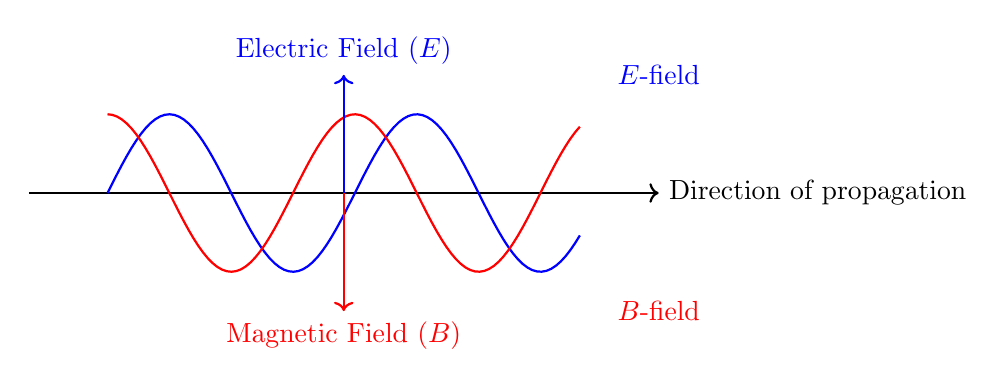
\begin{tikzpicture}[scale=1.0]
		% Wave propagation direction
		\draw[->, thick] (-1, 0) -- (7, 0) node[right] {Direction of propagation};

		% Electric field wave (in blue)
		\draw[blue, thick, domain=0:6, variable=\x, samples=100]
		plot ({\x}, {sin(2 * \x r)});
		\node[blue] at (7, 1.5) {$E$-field};

		% Magnetic field wave (in red)
		\draw[red, thick, domain=0:6, variable=\x, samples=100]
		plot ({\x}, {cos(2 * \x r)});
		\node[red] at (7, -1.5) {$B$-field};

		% Labels
		\draw[->, thick, blue] (3, 0) -- (3, 1.5) node[above] {Electric Field ($E$)};
		\draw[->, thick, red] (3, 0) -- (3, -1.5) node[below] {Magnetic Field ($B$)};
	\end{tikzpicture}
\end{center}

In this diagram, the electric field (\(E\)) oscillates in one plane, while the magnetic field (\(B\)) oscillates in a perpendicular plane. Both fields are sinusoidal and propagate together in the direction shown.

\section{The Wave Equation: \(c = f \lambda\)}

The relationship between the speed of light (\(c\)), the frequency (\(f\)), and the wavelength (\(\lambda\)) of an electromagnetic wave is given by the equation:
\[
	c = f \lambda
\]
where:
\begin{itemize}
	\item \(c\) is the speed of light in a vacuum, approximately \(3 \times 10^8\) m/s,
	\item \(f\) is the frequency of the wave (in Hz),
	\item \(\lambda\) is the wavelength of the wave (in meters).
\end{itemize}

This equation shows that the speed of light is the product of its frequency and wavelength. As the frequency of a wave increases, its wavelength decreases, and vice versa.

\section{The Electromagnetic Spectrum}

The electromagnetic spectrum encompasses all types of electromagnetic radiation, ranging from low-frequency radio waves to high-frequency gamma rays. Below is a diagram showing the range of the spectrum:

\begin{center}
	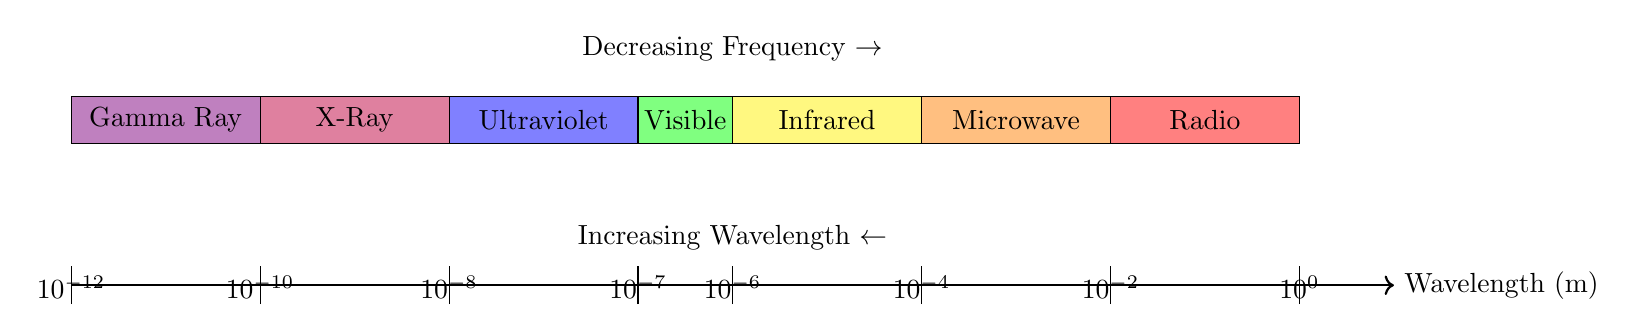
\begin{tikzpicture}[scale=1.2]
		% Spectrum axis

		% Spectrum sections (flipped)
		\draw[fill=violet!50] (0, 0.5) rectangle (2, 1) node[midway] {Gamma Ray};
		\draw[fill=purple!50] (2, 0.5) rectangle (4, 1) node[midway] {X-Ray};
		\draw[fill=blue!50] (4, 0.5) rectangle (6, 1) node[midway] {Ultraviolet};
		\draw[fill=green!50] (6, 0.5) rectangle (7, 1) node[midway] {Visible};
		\draw[fill=yellow!50] (7, 0.5) rectangle (9, 1) node[midway] {Infrared};
		\draw[fill=orange!50] (9, 0.5) rectangle (11, 1) node[midway] {Microwave};
		\draw[fill=red!50] (11, 0.5) rectangle (13, 1) node[midway] {Radio};

		% Labels for increasing frequency and decreasing wavelength
		\node at (7, 1.5) {Decreasing Frequency $\rightarrow$};
		\node at (7, -0.5) {Increasing Wavelength $\leftarrow$};

		% Wavelength ticks
		\draw[thick, ->] (0, -1) -- (14, -1) node[right] {Wavelength (m)};
		\draw (0, -1.2) -- (0, -0.8) node[below] {$10^{-12}$};
		\draw (2, -1.2) -- (2, -0.8) node[below] {$10^{-10}$};
		\draw (4, -1.2) -- (4, -0.8) node[below] {$10^{-8}$};
		\draw (6, -1.2) -- (6, -0.8) node[below] {$10^{-7}$};
		\draw (7, -1.2) -- (7, -0.8) node[below] {$10^{-6}$};
		\draw (9, -1.2) -- (9, -0.8) node[below] {$10^{-4}$};
		\draw (11, -1.2) -- (11, -0.8) node[below] {$10^{-2}$};
		\draw (13, -1.2) -- (13, -0.8) node[below] {$10^{0}$};
	\end{tikzpicture}
\end{center}

The electromagnetic spectrum ranges from long-wavelength, low-frequency waves like radio waves to short-wavelength, high-frequency waves like gamma rays. Visible light is a small portion of the spectrum, spanning from approximately 400 nm (violet) to 700 nm (red) in wavelength.

\section{Absorption Spectrum of Elements}

The absorption spectrum of an element is a unique pattern of dark lines or bands that appear when white light passes through a gas or vapor composed of the element. These dark lines correspond to specific wavelengths of light that have been absorbed by the element's atoms. Understanding absorption spectra is crucial in fields like astronomy and spectroscopy, as they allow scientists to identify elements in stars and distant galaxies.

\subsection{How Absorption Spectra Work}

When white light (which contains all visible wavelengths) passes through a sample of an element in its gaseous state, the electrons in the atoms of that element absorb specific amounts of energy. This energy corresponds to the difference between specific energy levels or orbits of the electrons.

When electrons absorb this energy, they jump from a lower energy level to a higher energy level, creating an absorption event. Each element has a unique set of energy levels, so the wavelengths absorbed (or "dark lines" in the spectrum) are also unique to each element. These dark lines are referred to as \textbf{absorption lines}.

\subsection{Relationship to Emission Spectrum}

The absorption spectrum is closely related to the \textbf{emission spectrum} of an element. When an electron drops from a higher energy level to a lower one, it emits light at a wavelength corresponding to the energy difference between these levels. In contrast, the absorption spectrum is formed when electrons move from lower to higher energy levels by absorbing light.

The emission lines and absorption lines occur at the same wavelengths for any given element, but they appear differently in the spectra:
\begin{itemize}
	\item \textbf{Emission Spectrum}: Bright lines on a dark background, representing wavelengths emitted by electrons falling to lower energy levels.
	\item \textbf{Absorption Spectrum}: Dark lines on a bright (continuous) background, representing wavelengths absorbed by electrons jumping to higher energy levels.
\end{itemize}

\subsection{Example: Hydrogen Absorption Spectrum}

The hydrogen atom, for example, has a simple absorption spectrum. It consists of a series of dark lines in the visible region, corresponding to the specific wavelengths absorbed by electrons as they move to higher energy levels. The Balmer series is a well-known part of hydrogen's absorption spectrum, with lines appearing in the visible light range.

Below is a simplified representation of the absorption spectrum of hydrogen:
\[
	\text{--- --- --- --- ---}
\]
The dark lines represent wavelengths absorbed by the hydrogen atoms.

\subsection{Applications of Absorption Spectra}

Absorption spectra are used in a variety of scientific fields to:
\begin{itemize}
	\item Identify elements present in stars and distant astronomical objects.
	\item Determine the chemical composition of substances.
	\item Study the energy levels and quantum mechanics of atoms and molecules.
\end{itemize}

Since each element has a unique absorption spectrum, this technique allows scientists to detect and analyze the presence of different elements based on the pattern of dark lines that appear in a spectrum.

\begin{center}
	
\begin{tikzpicture}[scale=1.0]
		% Continuous spectrum
		\shade[left color=white, right color=black] (0, 0) rectangle (10, 0.5);
		% Absorption lines
		\draw[very thick, white] (2, 0) -- (2, 0.5);
		\draw[very thick, white] (4, 0) -- (4, 0.5);
		\draw[very thick, white] (6, 0) -- (6, 0.5);
		\draw[very thick, white] (8, 0) -- (8, 0.5);
	\end{tikzpicture}
\end{center}

In this diagram, the gradient from white to black represents the continuous spectrum of light, while the vertical white lines represent absorption lines where specific wavelengths are absorbed by the element.

\section{Rydberg Equations and Emission Spectra}

The study of atomic emission spectra is crucial for understanding the quantized nature of energy levels within an atom. One of the fundamental equations used to describe the emission spectrum of hydrogen and similar atoms is the \textbf{Rydberg equation}. This equation predicts the wavelength of light emitted or absorbed when an electron transitions between different energy levels.

\subsection{Rydberg Equation}

The Rydberg equation is given by:
\[
	\frac{1}{\lambda} = R_H \left( \frac{1}{n_1^2} - \frac{1}{n_2^2} \right),
\]
where:
\begin{itemize}
	\item $\lambda$ is the wavelength of the emitted or absorbed photon.
	\item $R_H$ is the Rydberg constant for hydrogen, approximately $1.097 \times 10^7 \, \text{m}^{-1}$.
	\item $n_1$ and $n_2$ are the principal quantum numbers of the electron before and after the transition, with $n_2 > n_1$.
\end{itemize}

The equation essentially quantifies the relationship between the energy difference of two electron states and the wavelength of the photon emitted or absorbed during the electron's transition.

\subsection{Emission Spectrum of Hydrogen}

The emission spectrum of hydrogen is characterized by distinct lines, known as spectral lines, which correspond to the different possible transitions between energy levels in the atom. These series of lines are grouped into different spectral series based on the final quantum number $n_1$:
\begin{itemize}
	\item \textbf{Lyman series}: Transitions to $n_1 = 1$, resulting in ultraviolet radiation.
	\item \textbf{Balmer series}: Transitions to $n_1 = 2$, resulting in visible light.
	\item \textbf{Paschen series}: Transitions to $n_1 = 3$, resulting in infrared radiation.
\end{itemize}

Each spectral line within a series corresponds to a specific electron transition, and the wavelength of each line can be calculated using the Rydberg equation.

\subsection{Energy Levels and Photon Emission}

The energy difference between two quantum states in a hydrogen atom is given by:
\[
	\Delta E = E_{n_2} - E_{n_1} = -13.6 \, \text{eV} \left( \frac{1}{n_2^2} - \frac{1}{n_1^2} \right),
\]
where $-13.6 \, \text{eV}$ is the ground state energy of hydrogen. When an electron transitions from a higher energy state ($n_2$) to a lower one ($n_1$), a photon is emitted with energy:
\[
	E_{\text{photon}} = h \nu = \frac{hc}{\lambda},
\]
where:
\begin{itemize}
	\item $h$ is Planck’s constant ($6.626 \times 10^{-34} \, \text{Js}$).
	\item $\nu$ is the frequency of the photon.
	\item $c$ is the speed of light ($3.0 \times 10^8 \, \text{m/s}$).
\end{itemize}
By combining this with the Rydberg equation, one can relate the energy of the emitted photon to the observed wavelength of the spectral line.

\subsection{Applications of Rydberg Equation}

The Rydberg equation is not only crucial for predicting the emission spectrum of hydrogen but also for understanding other one-electron systems like He$^+$, Li$^{2+}$, and so forth. By studying the emission spectra of various elements, scientists can gain insights into the structure of atoms and the quantized nature of their energy levels. The emission spectra are also used in astrophysics to identify the elements present in distant stars and galaxies by comparing observed spectral lines with known values.

\section{Max Planck’s 1900 Theory and the Relationship $E = h\nu$}

In the early 1900s, Max Planck introduced a revolutionary concept that laid the foundation for quantum mechanics. To address the problem of blackbody radiation, Planck proposed that electromagnetic energy could only be emitted or absorbed in discrete units, or "quanta." This concept was a significant departure from classical physics and led to the development of the famous relationship:

\[
	E = h \nu,
\]

where:
\begin{itemize}
	\item $E$ is the energy of a quantum (or photon) of electromagnetic radiation.
	\item $h$ is Planck’s constant, with a value of approximately $6.626 \times 10^{-34} \, \text{Js}$.
	\item $\nu$ (or $f$) is the frequency of the electromagnetic radiation.
\end{itemize}

\subsection{The Blackbody Radiation Problem}

Classical physics predicted that a blackbody (an idealized physical body that absorbs all incident electromagnetic radiation) would emit radiation with an intensity that increases infinitely as the wavelength decreases (known as the “ultraviolet catastrophe”). However, experimental observations showed that the intensity reaches a peak and then drops off at shorter wavelengths. This discrepancy between theory and experiment led to the need for a new understanding of how radiation is emitted.

\subsection{Planck's Solution: Quantization of Energy}

Planck hypothesized that the energy emitted by a blackbody could only take on discrete values, rather than being continuous. He proposed that the energy of each quantum of radiation is proportional to its frequency, leading to the equation:
\[
	E = h \nu.
\]

This assumption meant that electromagnetic radiation is quantized and that the energy levels are spaced in multiples of $h \nu$. In essence, energy could only be emitted or absorbed in “packets” or quanta, not as a continuous wave.

\subsection{Implications of Planck's Theory}

Planck’s theory successfully explained the blackbody radiation spectrum, and the constant $h$, later known as Planck's constant, became a fundamental constant in quantum mechanics. This idea of quantization was groundbreaking because it introduced the concept that energy is not infinitely divisible, contradicting the classical wave theory of light.

The relationship $E = h \nu$ implies that higher frequency (shorter wavelength) radiation has more energy per photon. This paved the way for the development of quantum theory and influenced subsequent discoveries, including:
\begin{itemize}
	\item \textbf{Photoelectric Effect}: Albert Einstein used Planck’s concept to explain the photoelectric effect in 1905, showing that light can eject electrons from a material if the frequency is above a certain threshold. This provided further evidence of the particle-like behavior of light.
	\item \textbf{Wave-Particle Duality}: Planck’s work suggested that light exhibits both wave-like and particle-like properties, an idea that became central to quantum mechanics.
	\item \textbf{Quantum Energy Levels}: The concept of quantized energy levels led to the understanding of atomic structure and the development of quantum mechanical models, where electrons occupy discrete energy states around the nucleus.
\end{itemize}

\subsection{Applications and Further Developments}

Planck’s relationship, $E = h \nu$, has vast implications in various fields of physics and chemistry. It underpins the understanding of atomic spectra, molecular vibrations, and electronic transitions. It also plays a crucial role in technologies such as lasers, semiconductors, and quantum computing.

Overall, Planck’s introduction of the quantization of energy marked the beginning of a new era in physics, laying the groundwork for the development of quantum mechanics and fundamentally changing our understanding of the physical world.

\subsection{Quantized Emission Spectra}


\begin{center}
	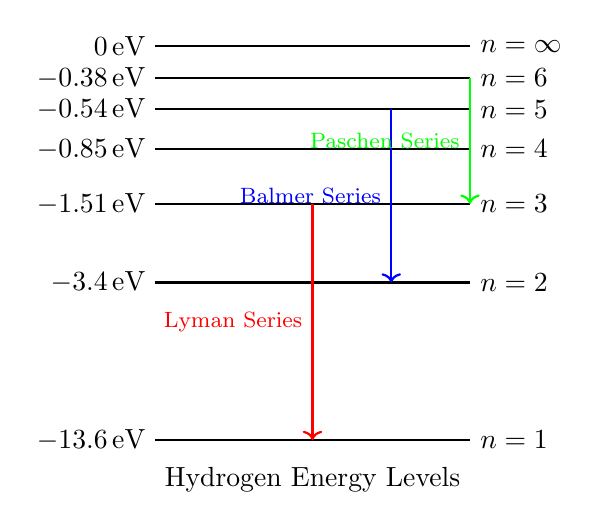
\begin{tikzpicture}
		% Draw the energy levels
		\draw[thick] (0,0) -- (4,0) node[right] {$n=1$};
		\draw[thick] (0,2) -- (4,2) node[right] {$n=2$};
		\draw[thick] (0,3) -- (4,3) node[right] {$n=3$};
		\draw[thick] (0,3.7) -- (4,3.7) node[right] {$n=4$};
		\draw[thick] (0,4.2) -- (4,4.2) node[right] {$n=5$};
		\draw[thick] (0,4.6) -- (4,4.6) node[right] {$n=6$};
		\draw[thick] (0,5) -- (4,5) node[right] {$n=\infty$};

		% Draw arrows indicating transitions
		\draw[->, thick, red] (2,3) -- (2,0) node[midway, left] {\footnotesize Lyman Series};
		\draw[->, thick, blue] (3,4.2) -- (3,2) node[midway, left] {\footnotesize Balmer Series};
		\draw[->, thick, green] (4,4.6) -- (4,3) node[midway, left] {\footnotesize Paschen Series};

		% Add energy labels
		\node[left] at (0,0) {$-13.6 \, \text{eV}$};
		\node[left] at (0,2) {$-3.4 \, \text{eV}$};
		\node[left] at (0,3) {$-1.51 \, \text{eV}$};
		\node[left] at (0,3.7) {$-0.85 \, \text{eV}$};
		\node[left] at (0,4.2) {$-0.54 \, \text{eV}$};
		\node[left] at (0,4.6) {$-0.38 \, \text{eV}$};
		\node[left] at (0,5) {$0 \, \text{eV}$};

		% Labels
		\node at (2,-0.5) {Hydrogen Energy Levels};
	\end{tikzpicture}
\end{center}

\section{The Photoelectric Effect}

The photoelectric effect is a phenomenon in which electrons are ejected from the surface of a material (usually a metal) when it is exposed to light of sufficient frequency. The experimental observations of the photoelectric effect could not be explained by classical wave theory and led to the development of quantum theory. Albert Einstein provided the explanation for this effect in 1905 by extending Max Planck's concept of quantization of energy.

\subsection{Einstein’s Explanation}

According to Einstein, light consists of packets of energy called "photons," each with an energy $E$ given by:
\[
	E = h f,
\]
where:
\begin{itemize}
	\item $h$ is Planck’s constant ($6.626 \times 10^{-34} \, \text{Js}$).
	\item $f$ is the frequency of the incident light.
\end{itemize}

When a photon hits the surface of a material, its energy is transferred to an electron. If the photon's energy is greater than a certain minimum energy needed to free the electron (known as the \textbf{work function} $\Phi$ of the material), the electron is ejected from the surface.

\subsection{The Photoelectric Equation}

The maximum kinetic energy $E_{\text{max}}$ of the ejected electron is given by the equation:
\[
	E_{\text{max}} = h f - \Phi,
\]
where:
\begin{itemize}
	\item $E_{\text{max}}$ is the maximum kinetic energy of the ejected electron.
	\item $h f$ is the energy of the incident photon.
	\item $\Phi$ is the work function of the material, which is the minimum energy required to free an electron from the surface.
\end{itemize}

This equation implies that the kinetic energy of the ejected electron depends linearly on the frequency of the incident light, and there is a threshold frequency $f_{\text{threshold}}$ below which no electrons are ejected, regardless of the intensity of the light.

\subsection{Stopping Voltage and Kinetic Energy}

The kinetic energy of the ejected electrons can be measured experimentally using a stopping voltage $V_s$. The stopping voltage is the voltage required to stop the ejected electrons from reaching the detector. The relationship between the stopping voltage and the kinetic energy is given by:
\[
	E_{\text{max}} = e V_s,
\]
where:
\begin{itemize}
	\item $e$ is the charge of the electron ($1.602 \times 10^{-19} \, \text{C}$).
	\item $V_s$ is the stopping voltage.
\end{itemize}

By measuring the stopping voltage for different frequencies of light, one can determine the work function $\Phi$ of the material and verify the linear relationship between $E_{\text{max}}$ and the frequency $f$ of the incident light.

\subsection{Significance of the Photoelectric Effect}

The photoelectric effect provided strong evidence for the quantization of light and supported the particle-like behavior of photons. This was a crucial step in the development of quantum mechanics. The effect also showed that the energy of ejected electrons is independent of the light’s intensity (which only affects the number of emitted electrons) and is instead solely dependent on the frequency of the incident light.

Applications of the photoelectric effect are found in various technologies, including photodetectors, solar cells, and photoelectron spectroscopy.

\subsection{Graph of Voltage vs. Kinetic Energy}

The photoelectric equation $E_{\text{max}} = h f - \Phi$ shows that the maximum kinetic energy of ejected electrons is linearly dependent on the frequency of the incident light. Experimentally, this relationship can be studied by plotting the stopping voltage $V_s$ (which is directly proportional to $E_{\text{max}}$) against the frequency $f$ of the incident light.


\begin{center}
	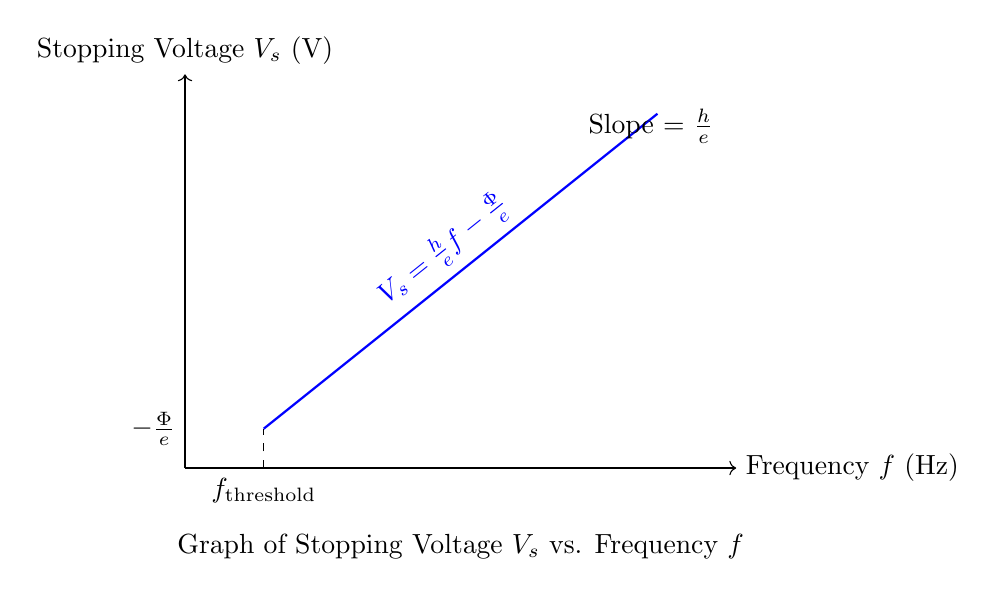
\begin{tikzpicture}
		% Axes
		\draw[->] (0,0) -- (7,0) node[right] {Frequency $f$ (Hz)};
		\draw[->] (0,0) -- (0,5) node[above] {Stopping Voltage $V_s$ (V)};

		% Line representing the photoelectric equation
		\draw[thick, blue] (1,0.5) -- (6,4.5) node[midway, above, sloped] {$V_s = \frac{h}{e}f - \frac{\Phi}{e}$};

		% Dots and line at threshold frequency
		\draw[dashed] (1,0) -- (1,0.5);
		\node[below] at (1,0) {$f_{\text{threshold}}$};

		% Labels for slope and intercept
		\node[above right] at (5,4) {Slope = $\frac{h}{e}$};
		\node[left] at (0,0.5) {$-\frac{\Phi}{e}$};

		% Label for graph
		\node at (3.5,-1) {Graph of Stopping Voltage $V_s$ vs. Frequency $f$};
	\end{tikzpicture}
\end{center}

\subsection{Explanation of the Graph}

The graph above represents the relationship between the stopping voltage $V_s$ and the frequency of the incident light $f$. The linear equation governing this relationship is:
\[
	V_s = \frac{h}{e} f - \frac{\Phi}{e},
\]
where:
\begin{itemize}
	\item $h$ is Planck’s constant.
	\item $e$ is the charge of an electron.
	\item $\Phi$ is the work function of the material.
\end{itemize}

In this graph:
\begin{itemize}
	\item The \textbf{slope} of the line is $\frac{h}{e}$. Since $h$ is Planck's constant and $e$ is a known constant (the electron charge), the slope provides a way to determine Planck's constant experimentally.
	\item The \textbf{y-intercept} is $-\frac{\Phi}{e}$, which corresponds to the work function of the material divided by the electron charge. This intercept is negative, as it represents the minimum energy needed to eject an electron.
	\item The point at which the line intersects the $f$-axis is the \textbf{threshold frequency} $f_{\text{threshold}}$. For frequencies below this value, no electrons are emitted because the photon's energy is insufficient to overcome the work function $\Phi$.
\end{itemize}

The linear nature of this graph is a direct consequence of the photoelectric effect and provides evidence for the quantization of energy in photons. By measuring the slope of this line, one can experimentally determine the value of Planck's constant $h$.

\section{Quantized Momentum of an Electron and Standing Waves in Orbits}

In the Bohr model of the atom, electrons are assumed to occupy discrete orbits around the nucleus. One of the key ideas is that the angular momentum of an electron in these orbits is quantized. Specifically, the angular momentum $L$ is given by:
\[
L = n \hbar,
\]
where:
\begin{itemize}
    \item $n$ is a positive integer (the principal quantum number).
    \item $\hbar$ is the reduced Planck's constant ($\hbar = \frac{h}{2\pi}$).
\end{itemize}

This quantization arises because the electron behaves as a standing wave in its orbit. For a stable orbit, the circumference of the orbit must be an integer multiple of the electron's wavelength $\lambda$:
\[
2 \pi r = n \lambda,
\]
where $r$ is the radius of the orbit.


\begin{center}
	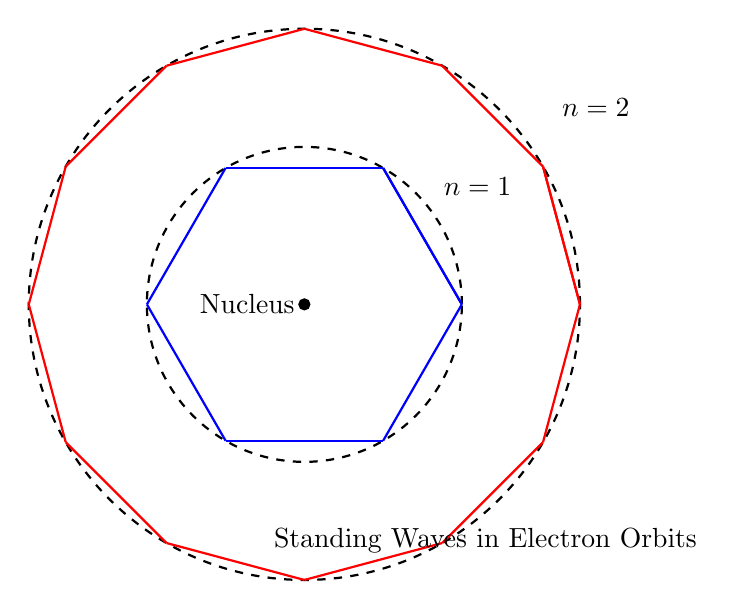
\begin{tikzpicture}
	    % Nucleus
	    \filldraw (0,0) circle (2pt) node[left] {Nucleus};
	
	    % Orbits
	    \draw[thick, dashed] (0,0) circle (2);
	    \draw[thick, dashed] (0,0) circle (3.5);
	    
	    % Standing wave in the first orbit (n=1)
	    \foreach \i in {0,60,...,360}
	        \draw[thick, blue] ({2*cos(\i)},{2*sin(\i)}) -- ({2*cos(\i+60)},{2*sin(\i+60)});
	    \node at (2.2,1.5) {$n=1$};
	    
	    % Standing wave in the second orbit (n=2)
	    \foreach \i in {0,30,...,360}
	        \draw[thick, red] ({3.5*cos(\i)},{3.5*sin(\i)}) -- ({3.5*cos(\i+30)},{3.5*sin(\i+30)});
	    \node at (3.7,2.5) {$n=2$};
	
	    % Labels
	    \node at (2.3,-3) {Standing Waves in Electron Orbits};
	\end{tikzpicture}
\end{center}

\subsection{Standing Waves and Quantized Orbits}

For each allowed orbit, the electron’s de Broglie wavelength $\lambda$ fits perfectly into the circumference of the orbit, creating a standing wave. This condition ensures that only specific, quantized orbits are possible, corresponding to different values of $n$. The quantization of angular momentum restricts electrons to these stable orbits, preventing them from spiraling into the nucleus.

In the diagram:
\begin{itemize}
    \item The dashed circles represent possible orbits.
    \item The blue and red standing waves correspond to $n=1$ and $n=2$, respectively, showing how the electron’s wave fits into each orbit.
\end{itemize}

\subsection{Radius of the Orbit of an Electron Around a Hydrogen Atom}

According to the Bohr model of the hydrogen atom, the radius of the electron’s orbit is quantized and given by the formula:
\[
r_n = \frac{n^2 \hbar^2}{k e^2 m_e} = n^2 a_0,
\]
where:
\begin{itemize}
    \item $r_n$ is the radius of the $n$-th orbit.
    \item $n$ is the principal quantum number ($n = 1, 2, 3, \ldots$).
    \item $\hbar$ is the reduced Planck's constant, given by $\hbar = \frac{h}{2\pi}$.
    \item $k$ is Coulomb’s constant, $k = \frac{1}{4 \pi \epsilon_0}$.
    \item $e$ is the elementary charge (the charge of an electron).
    \item $m_e$ is the mass of the electron.
    \item $a_0$ is the Bohr radius, defined as:
    \[
    a_0 = \frac{\hbar^2}{k e^2 m_e}.
    \]
\end{itemize}

The Bohr radius $a_0$ is approximately $5.29 \times 10^{-11} \, \text{m}$, which is the radius of the first orbit ($n = 1$) in a hydrogen atom. 

Thus, the radius of the $n$-th orbit is directly proportional to the square of the quantum number $n$, meaning that higher orbits are much larger than lower ones.
\subsection{Quantized Momentum of an Electron}

In the Bohr model of the atom, the momentum of an electron is quantized due to its wave-like nature. The electron behaves as a standing wave around the nucleus, and only certain orbits are allowed where the circumference of the orbit is an integer multiple of the electron's wavelength:
\[
2 \pi r = n \lambda,
\]
where $r$ is the radius of the orbit, $n$ is a positive integer (the principal quantum number), and $\lambda$ is the de Broglie wavelength of the electron.

Since the de Broglie wavelength is related to momentum $p$ by:
\[
\lambda = \frac{h}{p},
\]
the quantization condition becomes:
\[
p = \frac{n \hbar}{r},
\]
where $\hbar = \frac{h}{2\pi}$. This shows that the electron’s momentum is quantized, allowing only specific values for each orbit.


\end{document}